\section{What changed, and what the results can be used for}
\label{sec:synthesis}

The most consequential changes are changes in what the evidence licenses. Early numerical consistency became a demand for an explicit regulator and common current/stress definition. A finite matrix gap became a full-space statement only after controlling the representation tail. An appealing local inverse became a commutator identity with a retained boundary defect. A nonzero-variance Wilson probe became an identification problem after its slow response proved null. A formal retained semigroup became an implemented approximation only after the arithmetic error and the late-time ground component were controlled. These changes are useful even when the original parent objective remains open.

\subsection{From closed retained dynamics to complete channel loading}
For a self-adjoint generator $L$ and an orthogonal retained projection $P$, let
\begin{equation}
 A=PLP,\qquad B=QLP,\qquad D=QLQ,\qquad Q=I-P.
\end{equation}
Assume the domain and boundedness conditions used in the relevant projected problem. With $x=Pu$ and $y=Qu$, the exact heat equations are $x'=-Ax-B^*y$, $y'=-Bx-Dy$. Solving the second equation gives
\begin{equation}
 x'(t)=-Ax(t)-B^*e^{-tD}y(0)
       +\int_0^t B^*e^{-(t-s)D}Bx(s)\,\dd s.
\label{eq:memory-synthesis}
\end{equation}
This is the familiar projected-memory construction. The workbench contribution is its physical channel identification and controlled specialization, rather than invention of the formula. If $BP_{\rm old}=0$, initial leakage on an old subspace vanishes. It does not follow that $Be^{-tA}P_{\rm old}=0$: $A$ can load a new retained channel on which $B$ acts. AC2 exploits this delay quantitatively instead of deleting that channel.

Possible applications include certified reduced models for finite gauge systems, testing truncation designs, and preparing benchmarks for quantum-simulation algorithms. The practical advance is a bound on the full output, rather than convergence between two arbitrary finite cutoffs. A useful larger-graph application still requires a new complete basis, residual, and denominator calculation.

\subsection{From a useful heat bound to an executable all-time result}
The exact physical approximation and the finite-arithmetic approximation contribute different errors. On the declared normalized preparation class, suppose
\begin{equation}
 \norm{E(\sigma)x-E_P(\sigma)x}\le\varepsilon_{\rm phys},\quad
 \norm{E_P(\sigma)x-\widehat E_P(\sigma)x}\le\varepsilon_{\rm num},\quad
 \norm{E(\sigma)x}\ge d_0>0.
\end{equation}
The triangle inequality yields
\begin{equation}
 \frac{\norm{E(\sigma)x-\widehat E_P(\sigma)x}}
 {\norm{E(\sigma)x}}
 \le\frac{\varepsilon_{\rm phys}+\varepsilon_{\rm num}}{d_0}.
\label{eq:error-accounting}
\end{equation}
All three quantities need proof on the same input and time class. In particular, a relative theorem may fail when the true output decays to zero, even if an absolute theorem holds.

The all-time computational design addresses a second issue: a small error in a ground-energy shift causes secular drift. If an exact ground vector has energy $\mu$ but the program shifts by $\widehat\mu=\mu+\delta$, its ground component is multiplied by $e^{\delta\sigma}$. A fixed nonzero $\delta$ cannot support a uniform all-time guarantee. AF2 instead joins a certified finite-time polynomial evaluation to a certified ground projector with an exponentially bounded excited tail. The join is an algorithmic choice, not a new physical clock. Possible uses include long-heat-time state preparation, reproducible benchmark data, and testing alternative polynomial or rational approximations. None of these uses licenses real-time evolution without a separate theorem.

\subsection{From a source correction to a nonlinear stability problem}
An identity $[J,G]=-A+R$ with $\norm{R}<\norm{A}$ is useful evidence about the specified source $A$ and generator $G$. The next transformation generally changes both the source and the diagonal operator. A full iteration needs, for example, bounds on a declared map
\begin{equation}
 (G_n,A_n)\longmapsto (G_{n+1},A_{n+1},J_n)
\end{equation}
in one complete interaction norm, along with control of scalar and diagonal updates and the summability of the corrections. This display states a future obligation, not a derived recurrence. AE2 proves finite original weighted norms and per-source contraction in its smaller coupling region; it does not prove contraction of the collective weighted interaction. The distinction prevents an unsupported homogeneous numerical mass-gap claim.

The current construction may serve as a local preconditioner, an explicit approximate homological solver, or a starting point for a future stability iteration. Such applications are proposed mathematical uses; no faster numerical algorithm or new many-body phase has been measured here.

\subsection{From a resonant state to an informative observable}
An operator $B$ can prepare a state with nonzero variance while the selected averaged interaction annihilates that state. Then the selected slow readout is constant and cannot identify the slow parameter. AD1 supplies this control. AD2 uses actual six-cycle Wilson multiplication observables with nontrivial endpoints, retaining their own norms and higher moments. The distinction matters because a rank-one preparation surrogate and a multiplication operator may agree on $\Omega$ but differ elsewhere.

These results can inform the selection of mathematical test observables and simulation readouts. They do not demonstrate laboratory preparation, finite-resource feasibility at the sample physical clock, or a calibration connecting the summable model to the homogeneous model. The formula depends on the parameter combinations actually present; naming a frequency is not a measurement of an independent physical scale.

\subsection{Evidence networks and nonphysical geometry}
The released evidence network has 158 nodes and 260 directed links: 111 historical entries, 26 displayed equations, ten current loops, four premise nodes, and seven open targets. Its three edge types are source dependency, proposed transfer, and review selection. A source dependency records the declared use of a file or result; it is not necessarily a minimal mathematical dependency. Review-selection edges record chronology rather than logical implication. In particular, the drawing cannot close an edge labelled proposed transfer.

The grouped appendix and machine-readable ledgers make this network useful as a research-navigation and audit artifact. Figure~\ref{fig:network} shows its organization; node coordinates have no physical interpretation. A new calculation can be attached to the exact obstruction it addresses, while failed or limited outcomes remain visible.

\begin{figure}[htbp]\centering
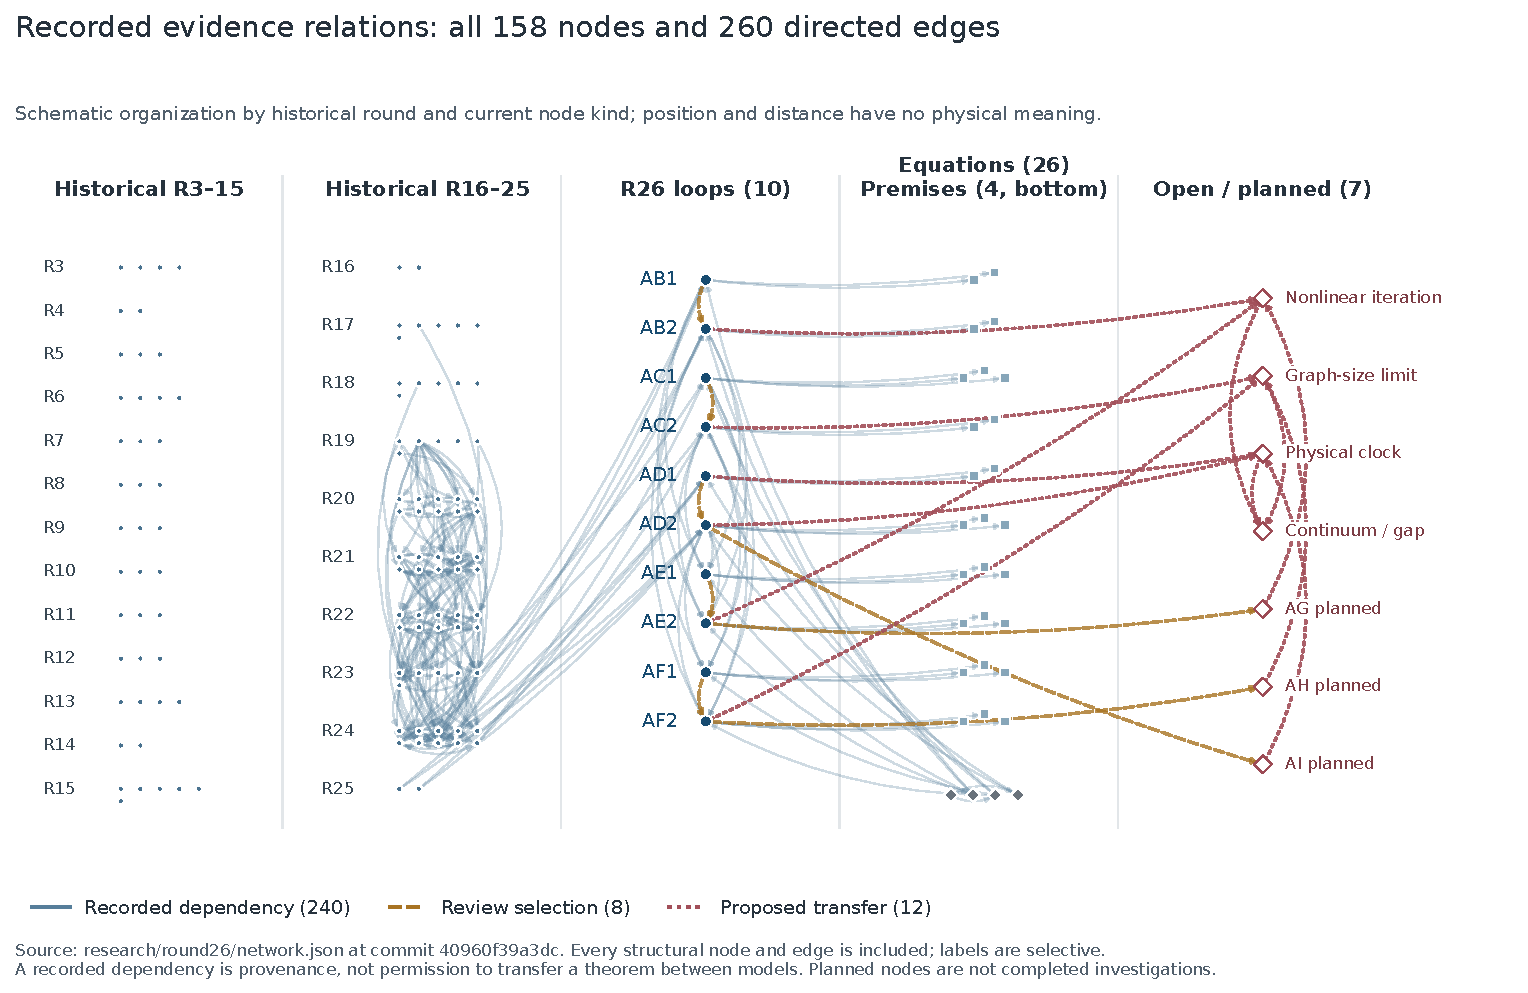
\includegraphics[width=\textwidth]{figures/network_structure.pdf}
\caption{The recorded evidence network, grouped for readability. Edges retain their audit meaning; geometric placement is a presentation choice. Open targets are not established conclusions.}
\label{fig:network}
\end{figure}
